%%%%%%%%%%%%%%%%%%%%%%%%%%%%%%%%%%%%%%%%%%%%%%%%%%%%%%%%%%%%%%%%%%%%%%%%%%%

\documentclass{standalone}

\usepackage{amsmath}
\usepackage{mathptmx}
\usepackage{pgfplots}
\usetikzlibrary{external}
\tikzexternalize{height-weight-scatterplot}
\pgfplotsset{compat=1.15}

%% IEEE uses Times Roman font, so we'll default to Times.
%% These three commands make up the entire times.sty package.
\renewcommand{\rmdefault}{ptm}
\renewcommand{\ttdefault}{pcr}
\normalfont\selectfont

\begin{document}

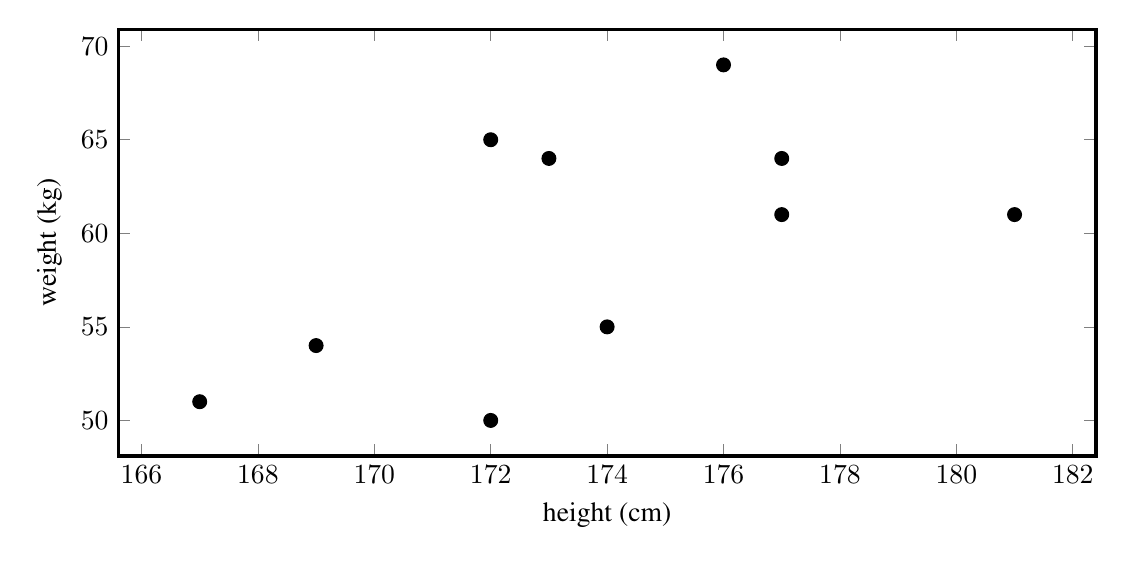
\begin{tikzpicture}
\tikzset{%%
  every mark/.append style={scale=1.0},%%
  scale=1.0%%
}
\pgfplotsset{%%
  every axis/.append style={font=\normalsize}%%
}
%%
\begin{axis}[%%
  axis line style=very thick,%%
  dotStyle/.style={only marks,mark size=2.5,black,mark color=black,mark=*},%%
  enlargelimits=true,%%
  height=7cm,%%
  width=14cm,%%
  xlabel={\normalsize height~(cm)},%%
  ylabel={\normalsize weight~(kg)}%%
]
%%
%%
\addplot[dotStyle] coordinates {
  (167,51)
  (181,61)
  (176,69)
  (173,64)
  (172,65)
  (174,55)
  (177,64)
  (177,61)
  (172,50)
  (169,54)
};
\end{axis}
\end{tikzpicture}

\end{document}
